\documentclass[12pt]{article}

\usepackage[margin=1in]{geometry}
\usepackage{graphicx}
\usepackage{fontspec}
\setmainfont[Ligatures=TeX,Mapping=tex-text,Numbers=OldStyle]{Adobe Garamond Pro}
\setsansfont[Numbers=OldStyle]{Roboto}
\setmonofont{Adobe Garamond Pro}
\usepackage{hyperref}
\usepackage[]{biblatex-chicago}
\addbibresource{bibliography.bib}

\begin{document}
\noindent Rachael Carlson \hfill \today\\
\noindent Reading Response 11\\
\noindent Music 314\\

% Several of this week's readings (Kristen, McSweeney, Ross) deal with
% the question of gender representation in the programming practices
% of art music institutions. In the discourse that these readings are
% drawn from, one of the key debates is over the methods that could be
% used to change the existing paradigms. Two of the most commonly
% asserted solutions are 1) to purposefully and aggressively program
% composers from underrepresented populations or 2) to focus on
% program newer music, with the assumption that the statistics with
% will even out based on the changing demographics of the pool of
% composers.

% Referring to specific ideas from these readings, briefly respond to
% this discourse, taking a stance if you have one, or outlining the
% key arguments in play.

\noindent Ross and Kirsten seem to be on the same page in regards to
the programming of new music and that music's relationship to
gender. They take the stance that if more new music is presented in
classical/art music venues the inequality of representation within the
world of new music will work itself out. I am not on this page. I wish
that this page was possible. I hope that we will find it to be
true. Especially given my desire for new works to be presented more
often than the oldies. I think that Ambrose's article straddles the
line between the two discourses noted in the prompt. It seems to me
that Ambrose is attempting to reveal the discrepancies between how a
woman is treated in an interview and how a man would be treated in a
similar interview. It seems to me that Ambrose's article is
essentially about how women are tokenized in an interview setting.

I think that both discourses can be reduced in the following way: 1)
recognition of gender identity and 2) denial of gender identity. These
discourses remind me of the discourses around race, namely, critical
race theory and colorblindness. The first asserts that race, though it
is a social construct, is fundamental to how people experience the
world; the second asserts that in a post-civil rights world, invoking
race serves no purpose, we have equality. The discourses which deny
social constructs seem to believe that equality already
exists.

Here is where I get into some of what ends up being considered my
politics. Personally, I think that equality is not as important as
equity. I am not interested in political freedom which can be
considered associated with the second discourse, the discourse of
denial. I am interested in social freedom of which the first discourse
might be associated. In order for there to be true equality we each
individual must have equity.


\begin{center}
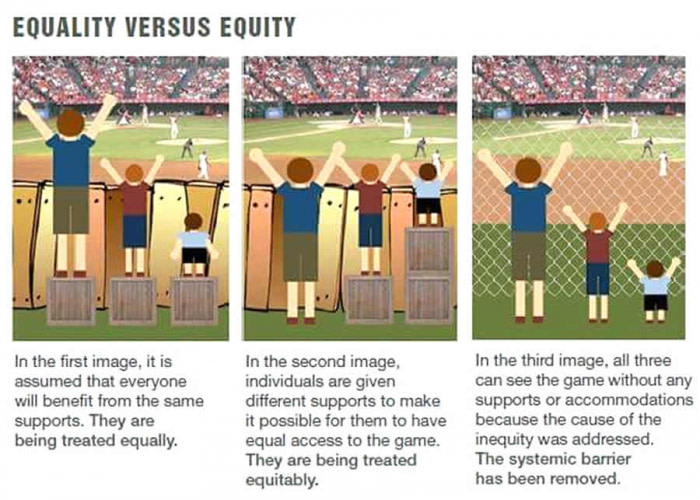
\includegraphics[width=0.5\textwidth]{equity.jpg}
\end{center}

\noindent This image sums up my view on the matter of equability quite
succinctly. I think that it highlights a discourse which is not
mentioned in these articles: what is causing this inequality? How can
we remove it? I think that Ross and Kirsten think that the amount of
new music premieres is the source of the barrier. Others might say
that the donors, those that are over 55 and seem to prefer the oldies,
are the barriers. However, when we remove those options, examples of
which are elucidated in McSweeney's article, the inequality remains. I
think that the question that we should be asking is ``what is the
barrier that is keeping composers of all backgrounds from equal
representation? My knee-jerk response would be capitalism; however,
there may be other barriers which might be easier to remove. I think
that I would be interested in examining the intersection between
gender studies, Marxism, and musicology. I think that it would reveal
some interesting avenues for discussion and contemplation. This would
be where we all wish that Adorno would have went in his analyses.

\pagenumbering{gobble}
\end{document}
%%% Local Variables:
%%% mode: latex
%%% TeX-master: t
%%% End:
